\providecommand{\main}{..}
\documentclass[../mthe-493-final-project.tex]{subfiles}

%Description of approach and final code-base architecture. Our physical model. Great place for an architecture diagram.

\begin{document}
    \chapter{Network Implementation}
    \label{ch:network-implementation}
    % Naive translation form math model to actual implementation.
    % e.g., workers are represented as machines on a network

    \section{}
    %% Appropriate tools
    % Potential tools, why were they looked at?
    % DCP and AXON
    To model the design problem and solution, appropriate tools are required. To represent workers, a set of devices capable of executing the computing tasks used in the application can be used. To facilitate the communication in the network, we need a framework to send and receive data. A computer program will need to run on each of the workers to complete tasks as they are received. These worker programs must record evaluation metrics and report the datum to a coordinator. A coordinator program will need to run on a device which will manage the program flow of benchmarking workers, optimizing data distribution, sending out work, aggregating results and finally recording metrics. There is also a requirement for the application to register presence of workers online, and the way to reach them.

    \section{}
    %% Evaluate tools (appropriatedness of selection)

    % Compare and constrast tool solutions
    % e.g. Explain cost aspect of implementation.
    The tools used to implement the network must meet some criteria.
    - Hardware must be cheap, simple to work with, and must be able to modify computation power
    - Communicate reliably
    - Generally able to implement constraints in spec
    - Implement cost as outlined in design
    - Communicate with limited unnecessary network delays
    - Record metrics accurately
    - Simple to fit to our application

    % Engineering tools/Evaluates tool limitations
    \subsection{DCP vs AXON}

    %% Application of tools
    \section{}

    \begin{figure}
        \centering
        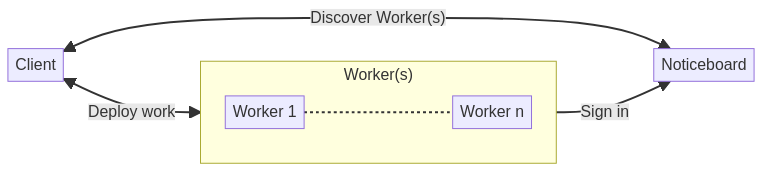
\includegraphics{network-1.png}
        \caption{Caption}
        \label{fig:network-flowchart}
    \end{figure}

    \begin{figure}
        \centering
        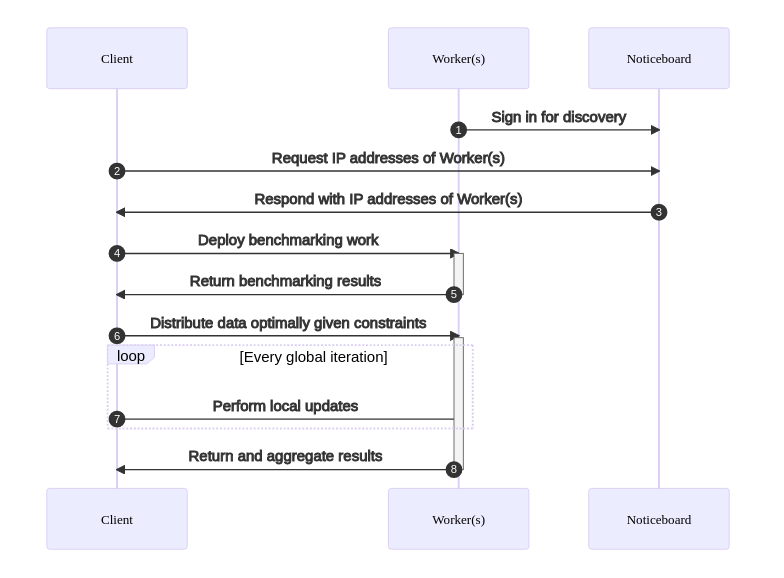
\includegraphics{network-2.png}
        \caption{Caption}
        \label{fig:network-sequence}
    \end{figure}

    % Diagrams n stuff
\end{document}
